\section{KULLANICI ARAYÜZÜ BİLEŞENLERİ}

Bu bölümde FaceScan AI uygulamasının kullanıcıya sunulan ekranları, her ekranın işlevsel bileşenleri ve uygulama içindeki veri akışı ayrıntılı biçimde açıklanmaktadır. Aşağıdaki ekran görüntüleri, uygulamanın gerçek cihaz üzerindeki çalışma ortamından alınmıştır.

\subsection{Açılış Ekranı ve Uygulama Logosu}

Uygulama ilk başlatıldığında, koyu arka plan üzerinde teal-cyan renk geçişleriyle tasarlanmış kalp ve EKG (elektrokardiyografi) dalgası ikonundan oluşan marka logosu animasyonlu olarak kullanıcıya sunulmaktadır. Bu açılış ekranı (splash screen), CSS keyframe animasyonlarıyla oluşturulmuş olup pulse (nabız atışı) efekti ve yukarıdan aşağıya doğru bir tarama hareketi içermektedir. Söz konusu tasarım tercihi, uygulamanın sağlık teknolojisi kimliğini ilk anda kullanıcıya hissettirmeyi hedeflemektedir.

\begin{figure}[h!]
    \centering
    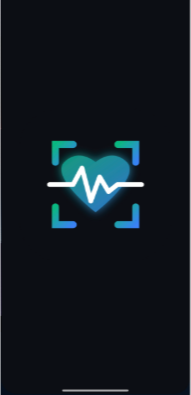
\includegraphics[width=0.35\linewidth]{sekil1_splash.png}
    \caption{FaceScan AI -- Açılış Animasyonu ve Uygulama Logosu}
    \label{fig:splash}
\end{figure}

\subsection{Ana Ekran (Dashboard) ve Kontrol Paneli}

Ana ekran (Dashboard), kullanıcı deneyiminin odak noktasını oluşturmaktadır. Üst kısımda \textbf{FaceScan AI} marka başlığı ve anlık bildirim ikonu yer almaktadır. Hemen altında uygulamanın temel çağrısını ifade eden \textit{"Yüz Tarayıcı Hazır"} başlıklı bir bilgi kartı bulunmaktadır; bu kart kameranın renk analizi yapacağını açıklayan kısa bir metni, "\%100 Yerel Veri Güvenliği" ve "Anlık İşlemci Analizi" olmak üzere iki temel özelliği simge-metin kombinasyonuyla listelemektedir.

Kartın hemen altında koyu arka plandan belirgin biçimde ayrışan gradient yeşil renkteki \textbf{Taramayı Başlat} butonu konumlandırılmıştır. Bu buton, Scanner ekranına geçişi tetiklemektedir. Ekranın orta bölümünde, günlük dönen sağlık hatırlatıcı kartı (Günün Sağlık Hatırlatıcısı) görüntülenmektedir; örnekte "Sarılık Belirtileri" konusunda kullanıcıyı bilgilendiren bir kart yer almaktadır. Son olarak "Geçmiş Analizler" bölümü, LocalStorage üzerinden okunan geçmiş tarama kayıtlarını tarih, risk seviyesi ve temel bulgularla birlikte listemektedir. Kullanıcı bu listede "Detaylar" butonuna basarak ilgili taramanın sonuçlarına erişebilmektedir.

\begin{figure}[h!]
    \centering
    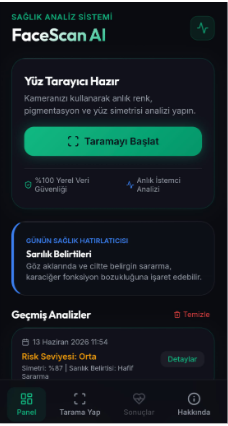
\includegraphics[width=0.55\linewidth]{sekil2_dashboard.png}
    \caption{FaceScan AI -- Ana Ekran: Taramayı Başlat Butonu, Günlük Sağlık Hatırlatıcısı ve Geçmiş Analizler}
    \label{fig:dashboard}
\end{figure}

\subsection{Kamera Tarayıcısı (Yüz Tarama) -- Hazır Durumu}

Kamera tarayıcısı ekranı, uygulamanın teknik çekirdeğini oluşturmaktadır. Ekran yüklendiğinde \texttt{navigator.mediaDevices.getUserMedia()} API'si çağrılarak kullanıcıdan kamera erişim izni istenmektedir \cite{webrtc2023spec}. İzin verilmesi durumunda canlı video akışı \texttt{<video>} öğesine bağlanmakta ve yüz hizalama halkası görünür hale gelmektedir.

Ekranın üst kısmında iki seçenek mevcuttur: \textbf{Canlı Kamera} ve \textbf{Fotoğraf Yükle}. Bu çift modlu yapı, hem gerçek zamanlı kamera akışıyla hem de galeriden seçilen statik görüntüyle analiz yapılabilmesine imkân tanımaktadır. Dairesel hizalama çerçevesi, kullanıcının yüzünü optimum konuma getirmesine yardımcı olurken ekranın alt kısmındaki \textbf{Fotoğrafı Analiz Et} butonu analizi başlatmaktadır.

\begin{figure}[h!]
    \centering
    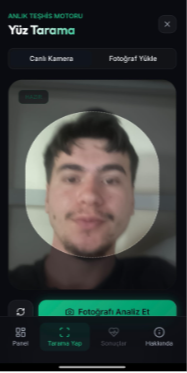
\includegraphics[width=0.55\linewidth]{sekil3_kamera_hazir.png}
    \caption{FaceScan AI -- Yüz Tarama Ekranı: Canlı Kamera Görüntüsü ve Hizalama Çerçevesi}
    \label{fig:kamera_hazir}
\end{figure}

\subsection{Kamera Tarayıcısı -- Analiz Aşaması}

Kullanıcı analizi başlattığında ekranın işlevsel davranışı değişmektedir. Yüz üzerinde tespit edilen anahtar noktalar (facial landmarks) mavi/mor renkli noktalar halinde görsel olarak işaretlenmektedir; bu noktalar göz köşeleri, burun ucu ve ağız kenarlarını temsil etmektedir. Ekranın alt kısmında durum mesajı güncellenerek \textit{"Cilt hemoglobin ve melanin dağılımı ölçülüyor..."} bilgisi kullanıcıya iletilmektedir. Bu aşamada Canvas API üzerinde piksel örneklemesi gerçekleşmekte ve HSL renk analizi algoritması devreye girmektedir.

\begin{figure}[h!]
    \centering
    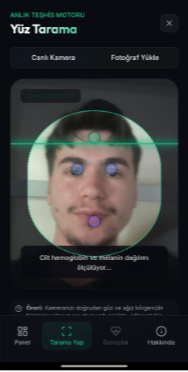
\includegraphics[width=0.55\linewidth]{sekil4_kamera_analiz.png}
    \caption{FaceScan AI -- Yüz Analizi Aşaması: Yüz Landmark Noktaları ve Anlık İşlem Bilgisi}
    \label{fig:kamera_analiz}
\end{figure}

\subsection{Teşhis Sonuçları (Tarama Sonuçları) Ekranı}

Analiz tamamlandığında kullanıcı otomatik olarak Tarama Sonuçları ekranına yönlendirilmektedir. Ekranın üst kısmında genel sağlık bulgusu metinsel olarak özetlenmektedir; örnekte \textbf{"Orta Derece Belirti"} tespiti, sarılık eğilimi ve renk sapmalarına dair kısa bir açıklamayla birlikte sunulmaktadır.

Ekranın alt yarısında \textbf{Bulgu Parametreleri} başlığı altında dört bağımsız dairesel ilerleme göstergesi (Circular Progress Indicator) yer almaktadır. Bu göstergeler saf SVG kodlarıyla oluşturulmuş olup dört temel ölçümü yansıtmaktadır:

\begin{itemize}
    \item \textbf{\%17 Sarılık Evresi:} Cilt piksellerindeki sarı ton dağılımının oranını göstermektedir; pembe renk çemberiyle temsil edilmektedir.
    \item \textbf{\%5 Oksijenizasyon:} Dudak çevresindeki kırmızı ton yoğunluğuna dayalı olarak hesaplanan oksijen doygunluk tahminini ifade etmektedir; mor renk çemberiyle gösterilmektedir.
    \item \textbf{\%6 Melanin Oranı:} Genel cilt tonu koyu renk oranını yansıtmaktadır; yeşil renk çemberiyle temsil edilmektedir.
    \item \textbf{\%80 Simetri:} Yüzün sol-sağ simetri indeksini göstermektedir; açık yeşil renk çemberiyle sunulmakta ve yüksek simetri değerinin sağlıklı bir kemik yapısına işaret ettiği belirtilmektedir.
\end{itemize}

\begin{figure}[h!]
    \centering
    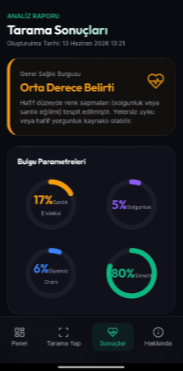
\includegraphics[width=0.55\linewidth]{sekil5_sonuclar.png}
    \caption{FaceScan AI -- Tarama Sonuçları: Orta Derece Belirti Tespiti ve Dört Parametreli Dairesel Göstergeler}
    \label{fig:sonuclar}
\end{figure}

\subsection{Alt Navigasyon Çubuğu}

Tüm ekranlarda sabit kalan alt navigasyon çubuğu dört sekme barındırmaktadır: \textbf{Panel} (Ana sayfa), \textbf{Tarama Yap}, \textbf{Sonuçlar} ve \textbf{Hakkında}. Aktif sekme teal rengiyle vurgulanmaktadır. Bu çubuğun tüm ekranlarda görünür kalması, kullanıcının uygulamanın herhangi bir noktasından diğer bölümlere tek dokunuşla geçiş yapabilmesini sağlamaktadır.

\subsection{Bulgu Detayları Ekranı}

Bulgu Detayları ekranı, Tarama Sonuçları panelinin detay kırılımını kullanıcıya sunmaktadır. Şekil \ref{fig:detaylar}'de görüldüğü üzere sklera analizi (hafif sararma), solgunluk analizi (normal), siyanoz analizi (normal) ve kas simetrisi (hafif asimetri) gibi ölçümler kartlar halinde listelenmektedir. Kartların altındaki açıklamalar, olası fizyolojik sebepleri (örneğin susuzluk veya tarama esnasındaki baş eğimi) açıklayarak kullanıcıyı bilgilendirir. Sayfa sonunda ayrıca sarı renkli bir "Akademik ve Tıbbi Feragatname" kartı yer almaktadır.

\begin{figure}[h!]
    \centering
    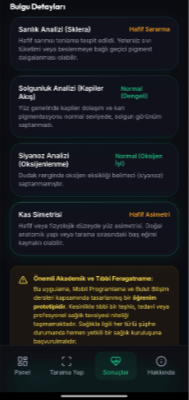
\includegraphics[width=0.55\linewidth]{sekil6_detaylar.png}
    \caption{FaceScan AI -- Bulgu Detayları ve Akademik Feragatname Kartı}
    \label{fig:detaylar}
\end{figure}

\subsection{Proje Bilgileri ve Hakkında Ekranı}

Uygulamanın "Hakkında" (Info) sekmesi, projenin akademik kapsamını, erişilebilirlik standartlarını, APK indirme linklerini ve geliştirici bilgilerini içerir. Şekil \ref{fig:hakkinda_1} ve Şekil \ref{fig:hakkinda_2}'de sunulan bu ekran, uygulamanın akademik teslim gereksinimlerini doğrudan yansıtmaktadır:

\begin{itemize}
    \item \textbf{Dönem Projesi Hakkında (Şekil \ref{fig:hakkinda_1}):} Projenin Mobil Programlama ve Bulut Bilişim dersleri kapsamındaki hedeflerini açıklar.
    \item \textbf{Tasarım ve Erişim Standartları (Şekil \ref{fig:hakkinda_2}):} Uygulamanın WCAG 2.1 standartlarına uygun olarak geliştirilen erişilebilirlik özelliklerini (ekran okuyucu uyumluluğu, yüksek kontrast oranı vb.) listeler.
    \item \textbf{APK ve Güvenlik Raporu Bağlantıları (Şekil \ref{fig:hakkinda_2}):} Kullanıcının hibrit Android uygulamasını (.apk) indirmesini ve MobSF güvenlik taraması sonuçlarını PDF olarak incelemesini sağlayan butonları barındırır.
\end{itemize}

\begin{figure}[h!]
    \centering
    \begin{subfigure}[b]{0.45\linewidth}
        \centering
        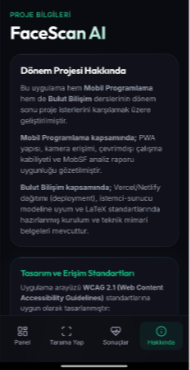
\includegraphics[width=\linewidth]{sekil7_hakkinda_1.png}
        \caption{Dönem Projesi Bilgileri}
        \label{fig:hakkinda_1}
    \end{subfigure}
    \hfill
    \begin{subfigure}[b]{0.45\linewidth}
        \centering
        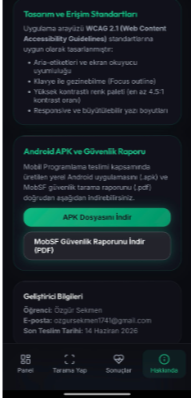
\includegraphics[width=\linewidth]{sekil8_hakkinda_2.png}
        \caption{Erişilebilirlik ve APK İndirme}
        \label{fig:hakkinda_2}
    \end{subfigure}
    \caption{FaceScan AI -- Proje Bilgileri ve Hakkında Sekmesi Detayları}
    \label{fig:hakkinda_genel}
\end{figure}

\subsection{Tıbbi Uyarı ve Sorumluluk Reddi Penceresi}

Sağlık alanında çalışan yapay zeka prototiplerinin yasal ve etik sorumlulukları gereğince, uygulamanın çeşitli bölümlerinde belirgin bir "Tıbbi Uyarı" kartı yer almaktadır. Şekil \ref{fig:tibbi_uyari}'de gösterilen bu kart, elde edilen analiz sonuçlarının kesin bir tıbbi tanı niteliği taşımadığını ve sağlık sorunları durumunda mutlaka uzman bir hekime başvurulması gerektiğini hatırlatarak sorumluluk sınırlarını netleştirmektedir.

\begin{figure}[h!]
    \centering
    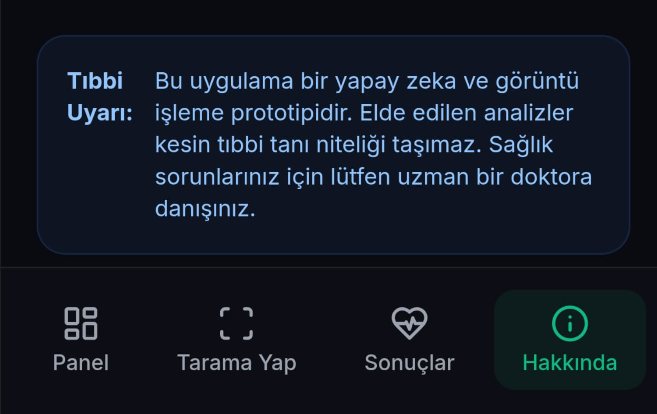
\includegraphics[width=0.55\linewidth]{sekil9_tibbi_uyari.png}
    \caption{FaceScan AI -- Tıbbi Uyarı ve Sorumluluk Reddi Mesajı}
    \label{fig:tibbi_uyari}
\end{figure}

